\documentclass[a4paper,12pt,exos,firamath]{nsi}

\documentclass[a4paper,12pt,cours,firamath]{nsi}
		
\setminted{fontsize=\small}
\begin{document}
{\large\bfseries \scshape Nom Prénom : \makebox[6cm]{\dotfill}\hfill Heure de passage : \makebox[3cm]{\dotfill}\hfill\\
\vspace{2em}
\hrule
\vspace{2mm}
\begin{center}\titlefont\Huge\color{UGLiBlue} BTS SIO\\
	Sous-épreuve E22 \\ 
    Algorithmique appliquée\\
	Contrôle en Cours de Formation\end{center}
\vspace{2mm}
\hrule}
\vspace{2em}
\begin{encadrecolore}{Déroulement de l'épreuve }{UGLiOrange}
	Cette épreuve de Contrôle en cours de Formation (CCF) se déroule en trois étapes :
\begin{itemize}
	\item \textbf{\'Etape 1 : \'Ecrit (30 minutes)}\par
	Vous devez traiter la partie A du sujet. Pour cette partie, l'ordinateur est interdit mais la calculatrice est autorisée.\\
    
    \textbf{Vous inscrirez vos réponses dans le document réponse à la fin du sujet.}\\
    
    Les algorithmes à écrire peuvent être rédigés en \textbf{langage naturel} ou en \textsc{Python}	mais ni en \textsc{C\#} ni en \textsc{VB.Net}.\\
    
    \textbf{À la fin de l'étape 1, votre document réponse doit être remis à la personne surveillant l'épreuve.} Vous garderez le sujet.
    \item \textbf{\'Etape 2 : sur machine (30 minutes)}\par
	Vous devez traiter la partie B du sujet à l'aide d'un ordinateur. Le langage utilisé est celui travaillé dans l'année, à savoir \textsc{Python}.
	Vous sauvegarderez votre travail sur la clé USB fournie.\par 
	La durée totale pour effectuer les deux premières étapes est exactement d'une heure. \par
	\item \textbf{\'Etape 3 : oral (20 minutes au maximum)}\\
	Cette partie se déroule en deux temps. Tout d'abord, vous disposez de 10 minutes pour présenter votre travail de l'étape 2 puis, au cours des 10 minutes suivantes, un entretien permet de préciser votre démarche.
\end{itemize}	

\textbf{À la fin de l'épreuve le sujet devra être rendu à l'examinateur.}
\end{encadrecolore}
\newpage


\titre{Traitement d'images}
\classe{CCF Algo SIO}
\maketitle

Une image rectangulaire en noir et blanc peut être représentée par une liste de lignes qui sont des listes d'entiers compris entre 0 (pour le noir) et 255 (pour le blanc).\\
\begin{multicols}{2}
    Par exemple la liste suivante :
    \begin{minted}{python}
[[255, 255, 0, 128], 
 [255, 255, 0, 0],
 [204, 165, 128, 64]]
\end{minted}

    correspond à l'image ci-contre.
    \columnbreak
    \begin{center}
        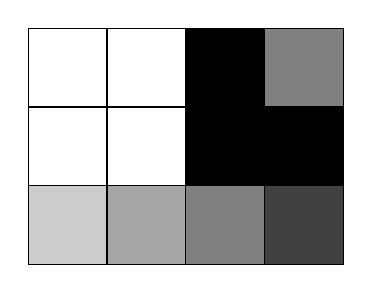
\begin{tikzpicture}
            \draw[fill=black!0] (0,2) rectangle (1,3);
            \draw[fill=black!0] (1,2) rectangle (2,3);
            \draw[fill=black!100] (2,2) rectangle (3,3);
            \draw[fill=black!50] (3,2) rectangle (4,3);
            \draw[fill=black!0] (0,1) rectangle (1,2);
            \draw[fill=black!0] (1,1) rectangle (2,2);
            \draw[fill=black!100] (2,1) rectangle (3,2);
            \draw[fill=black!100] (3,1) rectangle (4,2);
            \draw[fill=black!20] (0,0) rectangle (1,1);
            \draw[fill=black!35] (1,0) rectangle (2,1);
            \draw[fill=black!50] (2,0) rectangle (3,1);
            \draw[fill=black!75] (3,0) rectangle (4,1);
        \end{tikzpicture}
    \end{center}
\end{multicols}
\section*{\'Etape 1}

\begin{encadrecolore}{Question 1}{UGLiOrange}
    Si \mintinline{python}{lst} représente une image de $n$ lignes par $p$ colonnes.
    \begin{enumerate}
        \item	Quel est le nombre d'éléments de \mintinline{python}{lst} ?
        \item	Quel est le nombre d'éléments de \mintinline{python}{lst[0]} ?
    \end{enumerate}
\end{encadrecolore}

\begin{encadrecolore}{Question 2}{UGLiOrange}
    Compléter le code de la fonction \mintinline{python}{binarise} qui
    \begin{itemize}
        \item en entrée prend une liste représentant une image ;
        \item  modifie chaque pixel en mettant à 0 ceux qui sont inférieurs à 128 et à 255 ceux qui sont supérieurs.
    \end{itemize}

    \small
    \begin{verbatim}    
fonction binarise(lst)    
    variables
        i, j, n, p : entiers 
    n ← longueur(lst)
    p ← longueur(...)
    pour i allant de 0 à ...... faire
        ......
            si lst[i][j] < ... alors
                ...
            sinon 
                ...
        fin pour
    fin pour
    \end{verbatim}
    \normalsize
\end{encadrecolore}

\begin{encadrecolore}{Question}{UGLiOrange}
    Compléter le code de la fonction \mintinline{python}{cree_image_vide} qui
    \begin{itemize}
        \item en entrée prend deux entiers \mintinline{python}{n} et \mintinline{python}{p} ;
        \item renvoie une liste représentant une image « toute noire » de \mintinline{python}{n} lignes et \mintinline{python}{p} colonnes.
    \end{itemize}
    \begin{verbatim}    
fonction cree_image_vide(n, p)    
    variables
        i, j : entiers 
        resultat, ligne : liste
    resultat ← liste vide
    pour i allant de 0 à ... faire
        ligne ← ...
        pour j allant de 0 à ... faire
            ajouter 0 à la fin de ligne            
        fin pour
        ...
    fin pour
    ...
            \end{verbatim}
\end{encadrecolore}


On aimerait coder une fonction \mintinline{python}{miroir_vertical} qui
\begin{itemize}
    \item en entrée prend une liste \mintinline{python}{lst} représentant une image ;
    \item crée une liste vide aux mêmes dimensions que \mintinline{python}{lst} et remplit ses pixels en « renversant chaque ligne » ;
    \item renvoie cette liste.
\end{itemize}
Par exemple, en appliquant cette fonction à l'image de gauche, on doit obtenir celle de droite
\begin{center}
    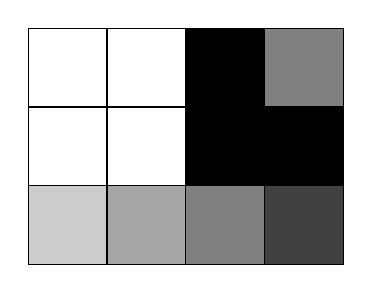
\begin{tikzpicture}
        \draw[fill=black!0] (0,2) rectangle (1,3);
        \draw[fill=black!0] (1,2) rectangle (2,3);
        \draw[fill=black!100] (2,2) rectangle (3,3);
        \draw[fill=black!50] (3,2) rectangle (4,3);
        \draw[fill=black!0] (0,1) rectangle (1,2);
        \draw[fill=black!0] (1,1) rectangle (2,2);
        \draw[fill=black!100] (2,1) rectangle (3,2);
        \draw[fill=black!100] (3,1) rectangle (4,2);
        \draw[fill=black!20] (0,0) rectangle (1,1);
        \draw[fill=black!35] (1,0) rectangle (2,1);
        \draw[fill=black!50] (2,0) rectangle (3,1);
        \draw[fill=black!75] (3,0) rectangle (4,1);
    \end{tikzpicture}
    \hspace{3cm}
    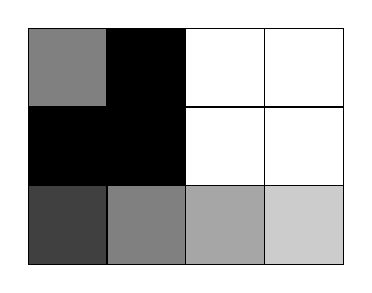
\begin{tikzpicture}
        \draw[fill=black!50] (0,2) rectangle (1,3);
        \draw[fill=black!100] (1,2) rectangle (2,3);
        \draw[fill=black!0] (2,2) rectangle (3,3);
        \draw[fill=black!0] (3,2) rectangle (4,3);
        \draw[fill=black!100] (0,1) rectangle (1,2);
        \draw[fill=black!100] (1,1) rectangle (2,2);
        \draw[fill=black!0] (2,1) rectangle (3,2);
        \draw[fill=black!0] (3,1) rectangle (4,2);
        \draw[fill=black!75] (0,0) rectangle (1,1);
        \draw[fill=black!50] (1,0) rectangle (2,1);
        \draw[fill=black!35] (2,0) rectangle (3,1);
        \draw[fill=black!20] (3,0) rectangle (4,1);
    \end{tikzpicture}
\end{center}
\begin{encadrecolore}{Question}{UGLiOrange}
    Compléter le code de la fonction \mintinline{python}{miroir_vertical}.

    \begin{verbatim}    
fonction cree_image_vide(lst)    
    variables
        i, j : entiers 
        resultat: liste
    n ← ...
    p ← ...
    resultat ← cree_image_vide(...)
    pour i allant de 0 à ... faire
        pour j allant de 0 à ... faire
            resultat[i][j] ← ...
        fin pour
    fin pour
    renvoyer resultat
    \end{verbatim}
\end{encadrecolore}

\section*{Étape 2}
\begin{encadrecolore}{Question}{UGLiOrange}
    Ouvrir le fichier \mintinline{python}{traitement_image.py} et coder les fonctions manquantes.
\end{encadrecolore}

\begin{encadrecolore}{Question}{UGLiOrange}
Coder la fonction \mintinline{python}{miroir_horizontal} qui
\begin{itemize}
\item en entrée prend une liste \mintinline{python}{lst} qui représente une image ;
\item renvoie une liste qui est l'image de \mintinline{python}{list} par une symétrie horizontale.
\end{itemize}
\end{encadrecolore}

\end{document}
